% SOURCE: RG_map_evidence_REFIX20260801.json :: cells.*.{gain, per_g."2".median_abs_drop_med3}; Spearman computed in-script (rank-level proxy; rho=0.81, p=4e-6)
% !TEX encoding = UTF-8 Unicode
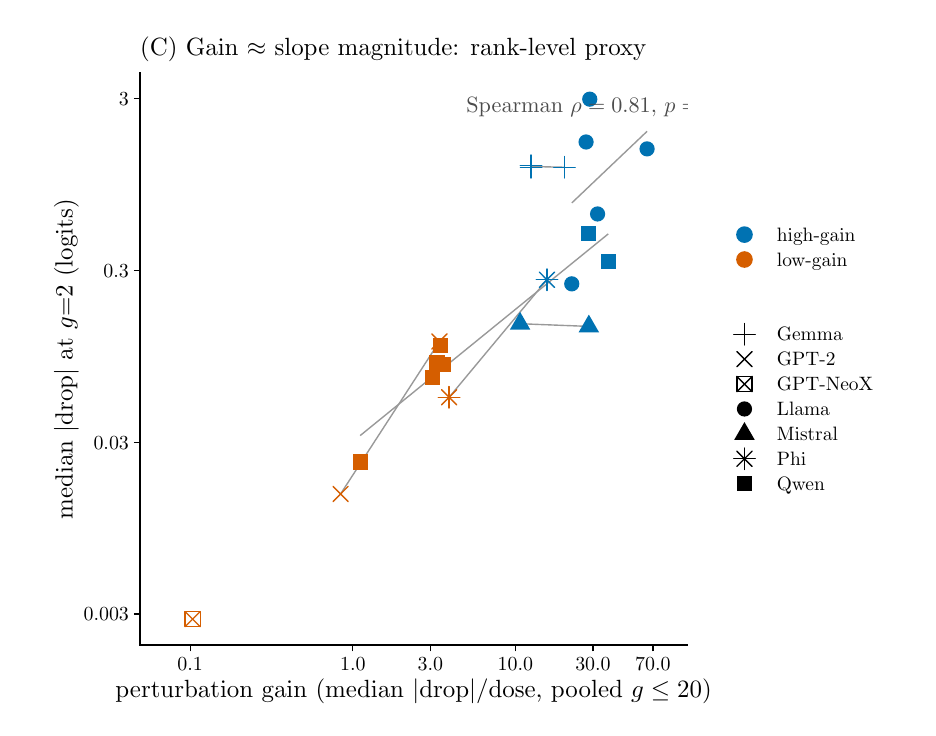
\begin{tikzpicture}[x=1pt,y=1pt]
\definecolor{fillColor}{RGB}{255,255,255}
\path[use as bounding box,fill=fillColor,fill opacity=0.00] (0,0) rectangle (317.99,245.72);
\begin{scope}
\path[clip] (  0.00,  0.00) rectangle (317.99,245.72);
\definecolor{drawColor}{RGB}{255,255,255}
\definecolor{fillColor}{RGB}{255,255,255}

\path[draw=drawColor,line width= 0.5pt,line join=round,line cap=round,fill=fillColor] ( -0.00,  0.00) rectangle (317.99,245.72);
\end{scope}
\begin{scope}
\path[clip] ( 40.64, 22.61) rectangle (238.29,229.27);
\definecolor{fillColor}{RGB}{255,255,255}

\path[fill=fillColor] ( 40.64, 22.61) rectangle (238.29,229.27);
\definecolor{drawColor}{gray}{0.60}

\path[draw=drawColor,line width= 0.5pt,line join=round] (181.90,195.55) --
	(182.05,195.55) --
	(182.20,195.55) --
	(182.36,195.54) --
	(182.51,195.54) --
	(182.66,195.54) --
	(182.81,195.53) --
	(182.97,195.53) --
	(183.12,195.52) --
	(183.27,195.52) --
	(183.42,195.52) --
	(183.58,195.51) --
	(183.73,195.51) --
	(183.88,195.51) --
	(184.03,195.50) --
	(184.19,195.50) --
	(184.34,195.50) --
	(184.49,195.49) --
	(184.64,195.49) --
	(184.80,195.49) --
	(184.95,195.48) --
	(185.10,195.48) --
	(185.26,195.48) --
	(185.41,195.47) --
	(185.56,195.47) --
	(185.71,195.47) --
	(185.87,195.46) --
	(186.02,195.46) --
	(186.17,195.46) --
	(186.32,195.45) --
	(186.48,195.45) --
	(186.63,195.45) --
	(186.78,195.44) --
	(186.93,195.44) --
	(187.09,195.44) --
	(187.24,195.43) --
	(187.39,195.43) --
	(187.54,195.43) --
	(187.70,195.42) --
	(187.85,195.42) --
	(188.00,195.42) --
	(188.15,195.41) --
	(188.31,195.41) --
	(188.46,195.41) --
	(188.61,195.40) --
	(188.76,195.40) --
	(188.92,195.40) --
	(189.07,195.39) --
	(189.22,195.39) --
	(189.37,195.39) --
	(189.53,195.38) --
	(189.68,195.38) --
	(189.83,195.38) --
	(189.98,195.37) --
	(190.14,195.37) --
	(190.29,195.37) --
	(190.44,195.36) --
	(190.59,195.36) --
	(190.75,195.36) --
	(190.90,195.35) --
	(191.05,195.35) --
	(191.20,195.34) --
	(191.36,195.34) --
	(191.51,195.34) --
	(191.66,195.33) --
	(191.81,195.33) --
	(191.97,195.33) --
	(192.12,195.32) --
	(192.27,195.32) --
	(192.42,195.32) --
	(192.58,195.31) --
	(192.73,195.31) --
	(192.88,195.31) --
	(193.03,195.30) --
	(193.19,195.30) --
	(193.34,195.30) --
	(193.49,195.29) --
	(193.64,195.29) --
	(193.80,195.29) --
	(193.95,195.28);

\path[draw=drawColor,line width= 0.5pt,line join=round] (113.08, 77.24) --
	(113.53, 77.94) --
	(113.98, 78.63) --
	(114.43, 79.33) --
	(114.88, 80.03) --
	(115.34, 80.73) --
	(115.79, 81.42) --
	(116.24, 82.12) --
	(116.69, 82.82) --
	(117.14, 83.52) --
	(117.60, 84.21) --
	(118.05, 84.91) --
	(118.50, 85.61) --
	(118.95, 86.30) --
	(119.40, 87.00) --
	(119.86, 87.70) --
	(120.31, 88.40) --
	(120.76, 89.09) --
	(121.21, 89.79) --
	(121.66, 90.49) --
	(122.12, 91.19) --
	(122.57, 91.88) --
	(123.02, 92.58) --
	(123.47, 93.28) --
	(123.92, 93.97) --
	(124.38, 94.67) --
	(124.83, 95.37) --
	(125.28, 96.07) --
	(125.73, 96.76) --
	(126.18, 97.46) --
	(126.64, 98.16) --
	(127.09, 98.86) --
	(127.54, 99.55) --
	(127.99,100.25) --
	(128.45,100.95) --
	(128.90,101.65) --
	(129.35,102.34) --
	(129.80,103.04) --
	(130.25,103.74) --
	(130.71,104.43) --
	(131.16,105.13) --
	(131.61,105.83) --
	(132.06,106.53) --
	(132.51,107.22) --
	(132.97,107.92) --
	(133.42,108.62) --
	(133.87,109.32) --
	(134.32,110.01) --
	(134.77,110.71) --
	(135.23,111.41) --
	(135.68,112.10) --
	(136.13,112.80) --
	(136.58,113.50) --
	(137.03,114.20) --
	(137.49,114.89) --
	(137.94,115.59) --
	(138.39,116.29) --
	(138.84,116.99) --
	(139.29,117.68) --
	(139.75,118.38) --
	(140.20,119.08) --
	(140.65,119.78) --
	(141.10,120.47) --
	(141.55,121.17) --
	(142.01,121.87) --
	(142.46,122.56) --
	(142.91,123.26) --
	(143.36,123.96) --
	(143.82,124.66) --
	(144.27,125.35) --
	(144.72,126.05) --
	(145.17,126.75) --
	(145.62,127.45) --
	(146.08,128.14) --
	(146.53,128.84) --
	(146.98,129.54) --
	(147.43,130.24) --
	(147.88,130.93) --
	(148.34,131.63) --
	(148.79,132.33);

\path[draw=drawColor,line width= 0.5pt,line join=round] (196.60,182.37) --
	(196.94,182.70) --
	(197.29,183.03) --
	(197.63,183.35) --
	(197.98,183.68) --
	(198.32,184.01) --
	(198.67,184.34) --
	(199.01,184.67) --
	(199.35,184.99) --
	(199.70,185.32) --
	(200.04,185.65) --
	(200.39,185.98) --
	(200.73,186.30) --
	(201.08,186.63) --
	(201.42,186.96) --
	(201.77,187.29) --
	(202.11,187.62) --
	(202.46,187.94) --
	(202.80,188.27) --
	(203.14,188.60) --
	(203.49,188.93) --
	(203.83,189.25) --
	(204.18,189.58) --
	(204.52,189.91) --
	(204.87,190.24) --
	(205.21,190.56) --
	(205.56,190.89) --
	(205.90,191.22) --
	(206.25,191.55) --
	(206.59,191.88) --
	(206.93,192.20) --
	(207.28,192.53) --
	(207.62,192.86) --
	(207.97,193.19) --
	(208.31,193.51) --
	(208.66,193.84) --
	(209.00,194.17) --
	(209.35,194.50) --
	(209.69,194.83) --
	(210.04,195.15) --
	(210.38,195.48) --
	(210.72,195.81) --
	(211.07,196.14) --
	(211.41,196.46) --
	(211.76,196.79) --
	(212.10,197.12) --
	(212.45,197.45) --
	(212.79,197.77) --
	(213.14,198.10) --
	(213.48,198.43) --
	(213.82,198.76) --
	(214.17,199.09) --
	(214.51,199.41) --
	(214.86,199.74) --
	(215.20,200.07) --
	(215.55,200.40) --
	(215.89,200.72) --
	(216.24,201.05) --
	(216.58,201.38) --
	(216.93,201.71) --
	(217.27,202.04) --
	(217.61,202.36) --
	(217.96,202.69) --
	(218.30,203.02) --
	(218.65,203.35) --
	(218.99,203.67) --
	(219.34,204.00) --
	(219.68,204.33) --
	(220.03,204.66) --
	(220.37,204.99) --
	(220.72,205.31) --
	(221.06,205.64) --
	(221.40,205.97) --
	(221.75,206.30) --
	(222.09,206.62) --
	(222.44,206.95) --
	(222.78,207.28) --
	(223.13,207.61) --
	(223.47,207.93) --
	(223.82,208.26);

\path[draw=drawColor,line width= 0.5pt,line join=round] (177.94,138.74) --
	(178.25,138.73) --
	(178.56,138.71) --
	(178.88,138.70) --
	(179.19,138.69) --
	(179.51,138.68) --
	(179.82,138.67) --
	(180.14,138.65) --
	(180.45,138.64) --
	(180.77,138.63) --
	(181.08,138.62) --
	(181.39,138.60) --
	(181.71,138.59) --
	(182.02,138.58) --
	(182.34,138.57) --
	(182.65,138.55) --
	(182.97,138.54) --
	(183.28,138.53) --
	(183.60,138.52) --
	(183.91,138.51) --
	(184.23,138.49) --
	(184.54,138.48) --
	(184.85,138.47) --
	(185.17,138.46) --
	(185.48,138.44) --
	(185.80,138.43) --
	(186.11,138.42) --
	(186.43,138.41) --
	(186.74,138.39) --
	(187.06,138.38) --
	(187.37,138.37) --
	(187.68,138.36) --
	(188.00,138.35) --
	(188.31,138.33) --
	(188.63,138.32) --
	(188.94,138.31) --
	(189.26,138.30) --
	(189.57,138.28) --
	(189.89,138.27) --
	(190.20,138.26) --
	(190.52,138.25) --
	(190.83,138.23) --
	(191.14,138.22) --
	(191.46,138.21) --
	(191.77,138.20) --
	(192.09,138.19) --
	(192.40,138.17) --
	(192.72,138.16) --
	(193.03,138.15) --
	(193.35,138.14) --
	(193.66,138.12) --
	(193.97,138.11) --
	(194.29,138.10) --
	(194.60,138.09) --
	(194.92,138.07) --
	(195.23,138.06) --
	(195.55,138.05) --
	(195.86,138.04) --
	(196.18,138.03) --
	(196.49,138.01) --
	(196.81,138.00) --
	(197.12,137.99) --
	(197.43,137.98) --
	(197.75,137.96) --
	(198.06,137.95) --
	(198.38,137.94) --
	(198.69,137.93) --
	(199.01,137.92) --
	(199.32,137.90) --
	(199.64,137.89) --
	(199.95,137.88) --
	(200.26,137.87) --
	(200.58,137.85) --
	(200.89,137.84) --
	(201.21,137.83) --
	(201.52,137.82) --
	(201.84,137.80) --
	(202.15,137.79) --
	(202.47,137.78) --
	(202.78,137.77);

\path[draw=drawColor,line width= 0.5pt,line join=round] (152.28,112.16) --
	(152.73,112.70) --
	(153.17,113.24) --
	(153.62,113.77) --
	(154.07,114.31) --
	(154.52,114.85) --
	(154.97,115.39) --
	(155.41,115.92) --
	(155.86,116.46) --
	(156.31,117.00) --
	(156.76,117.54) --
	(157.20,118.07) --
	(157.65,118.61) --
	(158.10,119.15) --
	(158.55,119.69) --
	(158.99,120.23) --
	(159.44,120.76) --
	(159.89,121.30) --
	(160.34,121.84) --
	(160.79,122.38) --
	(161.23,122.91) --
	(161.68,123.45) --
	(162.13,123.99) --
	(162.58,124.53) --
	(163.02,125.06) --
	(163.47,125.60) --
	(163.92,126.14) --
	(164.37,126.68) --
	(164.81,127.21) --
	(165.26,127.75) --
	(165.71,128.29) --
	(166.16,128.83) --
	(166.60,129.36) --
	(167.05,129.90) --
	(167.50,130.44) --
	(167.95,130.98) --
	(168.40,131.51) --
	(168.84,132.05) --
	(169.29,132.59) --
	(169.74,133.13) --
	(170.19,133.66) --
	(170.63,134.20) --
	(171.08,134.74) --
	(171.53,135.28) --
	(171.98,135.82) --
	(172.42,136.35) --
	(172.87,136.89) --
	(173.32,137.43) --
	(173.77,137.97) --
	(174.22,138.50) --
	(174.66,139.04) --
	(175.11,139.58) --
	(175.56,140.12) --
	(176.01,140.65) --
	(176.45,141.19) --
	(176.90,141.73) --
	(177.35,142.27) --
	(177.80,142.80) --
	(178.24,143.34) --
	(178.69,143.88) --
	(179.14,144.42) --
	(179.59,144.95) --
	(180.04,145.49) --
	(180.48,146.03) --
	(180.93,146.57) --
	(181.38,147.10) --
	(181.83,147.64) --
	(182.27,148.18) --
	(182.72,148.72) --
	(183.17,149.25) --
	(183.62,149.79) --
	(184.06,150.33) --
	(184.51,150.87) --
	(184.96,151.40) --
	(185.41,151.94) --
	(185.86,152.48) --
	(186.30,153.02) --
	(186.75,153.56) --
	(187.20,154.09) --
	(187.65,154.63);

\path[draw=drawColor,line width= 0.5pt,line join=round] (120.15, 98.32) --
	(121.28, 99.24) --
	(122.42,100.17) --
	(123.55,101.09) --
	(124.69,102.01) --
	(125.82,102.93) --
	(126.96,103.86) --
	(128.09,104.78) --
	(129.23,105.70) --
	(130.36,106.62) --
	(131.50,107.55) --
	(132.63,108.47) --
	(133.77,109.39) --
	(134.90,110.31) --
	(136.04,111.24) --
	(137.17,112.16) --
	(138.31,113.08) --
	(139.44,114.00) --
	(140.57,114.93) --
	(141.71,115.85) --
	(142.84,116.77) --
	(143.98,117.69) --
	(145.11,118.62) --
	(146.25,119.54) --
	(147.38,120.46) --
	(148.52,121.38) --
	(149.65,122.31) --
	(150.79,123.23) --
	(151.92,124.15) --
	(153.06,125.07) --
	(154.19,126.00) --
	(155.33,126.92) --
	(156.46,127.84) --
	(157.59,128.76) --
	(158.73,129.69) --
	(159.86,130.61) --
	(161.00,131.53) --
	(162.13,132.45) --
	(163.27,133.38) --
	(164.40,134.30) --
	(165.54,135.22) --
	(166.67,136.14) --
	(167.81,137.07) --
	(168.94,137.99) --
	(170.08,138.91) --
	(171.21,139.83) --
	(172.35,140.76) --
	(173.48,141.68) --
	(174.62,142.60) --
	(175.75,143.52) --
	(176.88,144.45) --
	(178.02,145.37) --
	(179.15,146.29) --
	(180.29,147.21) --
	(181.42,148.14) --
	(182.56,149.06) --
	(183.69,149.98) --
	(184.83,150.90) --
	(185.96,151.83) --
	(187.10,152.75) --
	(188.23,153.67) --
	(189.37,154.59) --
	(190.50,155.52) --
	(191.64,156.44) --
	(192.77,157.36) --
	(193.91,158.28) --
	(195.04,159.21) --
	(196.17,160.13) --
	(197.31,161.05) --
	(198.44,161.97) --
	(199.58,162.90) --
	(200.71,163.82) --
	(201.85,164.74) --
	(202.98,165.66) --
	(204.12,166.58) --
	(205.25,167.51) --
	(206.39,168.43) --
	(207.52,169.35) --
	(208.66,170.27) --
	(209.79,171.20);
\definecolor{fillColor}{RGB}{0,114,178}

\path[fill=fillColor] (196.60,153.15) circle (  2.75);

\path[fill=fillColor] (201.78,204.41) circle (  2.75);

\path[fill=fillColor] (203.11,219.88) circle (  2.75);

\path[fill=fillColor] (223.82,201.92) circle (  2.75);

\path[fill=fillColor] (205.93,178.40) circle (  2.75);

\path[fill=fillColor] (202.78,142.04) --
	(206.48,135.63) --
	(199.08,135.63) --
	cycle;

\path[fill=fillColor] (177.94,143.01) --
	(181.63,136.60) --
	(174.24,136.60) --
	cycle;
\definecolor{drawColor}{RGB}{0,114,178}

\path[draw=drawColor,line width= 0.5pt,line join=round,line cap=round] (184.90,151.88) -- (190.39,157.38);

\path[draw=drawColor,line width= 0.5pt,line join=round,line cap=round] (184.90,157.38) -- (190.39,151.88);

\path[draw=drawColor,line width= 0.5pt,line join=round,line cap=round] (183.76,154.63) -- (191.53,154.63);

\path[draw=drawColor,line width= 0.5pt,line join=round,line cap=round] (187.65,150.75) -- (187.65,158.52);
\definecolor{drawColor}{RGB}{213,94,0}

\path[draw=drawColor,line width= 0.5pt,line join=round,line cap=round] (149.53,109.41) -- (155.03,114.91);

\path[draw=drawColor,line width= 0.5pt,line join=round,line cap=round] (149.53,114.91) -- (155.03,109.41);

\path[draw=drawColor,line width= 0.5pt,line join=round,line cap=round] (148.39,112.16) -- (156.16,112.16);

\path[draw=drawColor,line width= 0.5pt,line join=round,line cap=round] (152.28,108.28) -- (152.28,116.05);

\path[fill=fillColor] (199.90,168.69) --
	(205.40,168.69) --
	(205.40,174.18) --
	(199.90,174.18) --
	cycle;
\definecolor{fillColor}{RGB}{213,94,0}

\path[fill=fillColor] (145.19,121.81) --
	(150.69,121.81) --
	(150.69,127.30) --
	(145.19,127.30) --
	cycle;

\path[fill=fillColor] (117.40, 86.01) --
	(122.90, 86.01) --
	(122.90, 91.51) --
	(117.40, 91.51) --
	cycle;

\path[fill=fillColor] (143.62,116.47) --
	(149.12,116.47) --
	(149.12,121.96) --
	(143.62,121.96) --
	cycle;
\definecolor{fillColor}{RGB}{0,114,178}

\path[fill=fillColor] (207.04,158.59) --
	(212.54,158.59) --
	(212.54,164.08) --
	(207.04,164.08) --
	cycle;
\definecolor{fillColor}{RGB}{213,94,0}

\path[fill=fillColor] (147.60,121.25) --
	(153.09,121.25) --
	(153.09,126.74) --
	(147.60,126.74) --
	cycle;

\path[fill=fillColor] (146.35,128.15) --
	(151.84,128.15) --
	(151.84,133.64) --
	(146.35,133.64) --
	cycle;
\definecolor{drawColor}{RGB}{0,114,178}

\path[draw=drawColor,line width= 0.5pt,line join=round,line cap=round] (190.06,195.28) -- (197.83,195.28);

\path[draw=drawColor,line width= 0.5pt,line join=round,line cap=round] (193.95,191.40) -- (193.95,199.17);

\path[draw=drawColor,line width= 0.5pt,line join=round,line cap=round] (178.01,195.83) -- (185.78,195.83);

\path[draw=drawColor,line width= 0.5pt,line join=round,line cap=round] (181.90,191.95) -- (181.90,199.72);

\path[draw=drawColor,line width= 0.5pt,line join=round,line cap=round] (178.03,195.27) -- (185.80,195.27);

\path[draw=drawColor,line width= 0.5pt,line join=round,line cap=round] (181.92,191.39) -- (181.92,199.16);
\definecolor{drawColor}{RGB}{213,94,0}

\path[draw=drawColor,line width= 0.5pt,line join=round,line cap=round] ( 56.86, 29.25) rectangle ( 62.35, 34.75);

\path[draw=drawColor,line width= 0.5pt,line join=round,line cap=round] ( 56.86, 29.25) -- ( 62.35, 34.75);

\path[draw=drawColor,line width= 0.5pt,line join=round,line cap=round] ( 56.86, 34.75) -- ( 62.35, 29.25);

\path[draw=drawColor,line width= 0.5pt,line join=round,line cap=round] (146.04,129.58) -- (151.53,135.07);

\path[draw=drawColor,line width= 0.5pt,line join=round,line cap=round] (146.04,135.07) -- (151.53,129.58);

\path[draw=drawColor,line width= 0.5pt,line join=round,line cap=round] (110.33, 74.49) -- (115.82, 79.99);

\path[draw=drawColor,line width= 0.5pt,line join=round,line cap=round] (110.33, 79.99) -- (115.82, 74.49);
\definecolor{drawColor}{gray}{0.30}

\node[text=drawColor,anchor=base west,inner sep=0pt, outer sep=0pt, scale=  0.80] at (158.55,214.89) {Spearman $\rho = 0.81$, $p = 4.1e-06$};
\end{scope}
\begin{scope}
\path[clip] (  0.00,  0.00) rectangle (317.99,245.72);
\definecolor{drawColor}{RGB}{0,0,0}

\path[draw=drawColor,line width= 0.5pt,line join=round,line cap=rect] ( 40.64, 22.61) --
	( 40.64,229.27);
\end{scope}
\begin{scope}
\path[clip] (  0.00,  0.00) rectangle (317.99,245.72);
\definecolor{drawColor}{RGB}{0,0,0}

\node[text=drawColor,anchor=base east,inner sep=0pt, outer sep=0pt, scale=  0.72] at ( 36.59, 31.38) {0.003};

\node[text=drawColor,anchor=base east,inner sep=0pt, outer sep=0pt, scale=  0.72] at ( 36.59, 93.44) {0.03};

\node[text=drawColor,anchor=base east,inner sep=0pt, outer sep=0pt, scale=  0.72] at ( 36.59,155.50) {0.3};

\node[text=drawColor,anchor=base east,inner sep=0pt, outer sep=0pt, scale=  0.72] at ( 36.59,217.57) {3};
\end{scope}
\begin{scope}
\path[clip] (  0.00,  0.00) rectangle (317.99,245.72);
\definecolor{drawColor}{RGB}{0,0,0}

\path[draw=drawColor,line width= 0.5pt,line join=round] ( 38.39, 33.86) --
	( 40.64, 33.86);

\path[draw=drawColor,line width= 0.5pt,line join=round] ( 38.39, 95.92) --
	( 40.64, 95.92);

\path[draw=drawColor,line width= 0.5pt,line join=round] ( 38.39,157.98) --
	( 40.64,157.98);

\path[draw=drawColor,line width= 0.5pt,line join=round] ( 38.39,220.05) --
	( 40.64,220.05);
\end{scope}
\begin{scope}
\path[clip] (  0.00,  0.00) rectangle (317.99,245.72);
\definecolor{drawColor}{RGB}{0,0,0}

\path[draw=drawColor,line width= 0.5pt,line join=round,line cap=rect] ( 40.64, 22.61) --
	(238.29, 22.61);
\end{scope}
\begin{scope}
\path[clip] (  0.00,  0.00) rectangle (317.99,245.72);
\definecolor{drawColor}{RGB}{0,0,0}

\path[draw=drawColor,line width= 0.5pt,line join=round] ( 58.73, 20.36) --
	( 58.73, 22.61);

\path[draw=drawColor,line width= 0.5pt,line join=round] (117.48, 20.36) --
	(117.48, 22.61);

\path[draw=drawColor,line width= 0.5pt,line join=round] (145.52, 20.36) --
	(145.52, 22.61);

\path[draw=drawColor,line width= 0.5pt,line join=round] (176.24, 20.36) --
	(176.24, 22.61);

\path[draw=drawColor,line width= 0.5pt,line join=round] (204.27, 20.36) --
	(204.27, 22.61);

\path[draw=drawColor,line width= 0.5pt,line join=round] (225.89, 20.36) --
	(225.89, 22.61);
\end{scope}
\begin{scope}
\path[clip] (  0.00,  0.00) rectangle (317.99,245.72);
\definecolor{drawColor}{RGB}{0,0,0}

\node[text=drawColor,anchor=base,inner sep=0pt, outer sep=0pt, scale=  0.72] at ( 58.73, 13.60) {0.1};

\node[text=drawColor,anchor=base,inner sep=0pt, outer sep=0pt, scale=  0.72] at (117.48, 13.60) {1.0};

\node[text=drawColor,anchor=base,inner sep=0pt, outer sep=0pt, scale=  0.72] at (145.52, 13.60) {3.0};

\node[text=drawColor,anchor=base,inner sep=0pt, outer sep=0pt, scale=  0.72] at (176.24, 13.60) {10.0};

\node[text=drawColor,anchor=base,inner sep=0pt, outer sep=0pt, scale=  0.72] at (204.27, 13.60) {30.0};

\node[text=drawColor,anchor=base,inner sep=0pt, outer sep=0pt, scale=  0.72] at (225.89, 13.60) {70.0};
\end{scope}
\begin{scope}
\path[clip] (  0.00,  0.00) rectangle (317.99,245.72);
\definecolor{drawColor}{RGB}{0,0,0}

\node[text=drawColor,anchor=base,inner sep=0pt, outer sep=0pt, scale=  0.90] at (139.46,  3.75) {perturbation gain (median $|$drop$|$/dose, pooled $g\leq20$)};
\end{scope}
\begin{scope}
\path[clip] (  0.00,  0.00) rectangle (317.99,245.72);
\definecolor{drawColor}{RGB}{0,0,0}

\node[text=drawColor,rotate= 90.00,anchor=base,inner sep=0pt, outer sep=0pt, scale=  0.90] at ( 16.20,125.94) {median $|$drop$|$ at $g{=}2$ (logits)};
\end{scope}
\begin{scope}
\path[clip] (  0.00,  0.00) rectangle (317.99,245.72);
\definecolor{fillColor}{RGB}{255,255,255}

\path[fill=fillColor] (247.29,152.94) rectangle (303.62,179.94);
\end{scope}
\begin{scope}
\path[clip] (  0.00,  0.00) rectangle (317.99,245.72);
\definecolor{fillColor}{RGB}{255,255,255}

\path[fill=fillColor] (251.79,166.44) rectangle (266.24,175.44);
\definecolor{drawColor}{RGB}{0,114,178}
\definecolor{fillColor}{RGB}{0,114,178}

\path[draw=drawColor,line width= 0.5pt,line join=round,line cap=round,fill=fillColor] (259.01,170.94) circle (  2.75);
\end{scope}
\begin{scope}
\path[clip] (  0.00,  0.00) rectangle (317.99,245.72);
\definecolor{fillColor}{RGB}{255,255,255}

\path[fill=fillColor] (251.79,157.44) rectangle (266.24,166.44);
\definecolor{drawColor}{RGB}{213,94,0}
\definecolor{fillColor}{RGB}{213,94,0}

\path[draw=drawColor,line width= 0.5pt,line join=round,line cap=round,fill=fillColor] (259.01,161.94) circle (  2.75);
\end{scope}
\begin{scope}
\path[clip] (  0.00,  0.00) rectangle (317.99,245.72);
\definecolor{drawColor}{RGB}{0,0,0}

\node[text=drawColor,anchor=base west,inner sep=0pt, outer sep=0pt, scale=  0.70] at (270.74,168.53) {high-gain};
\end{scope}
\begin{scope}
\path[clip] (  0.00,  0.00) rectangle (317.99,245.72);
\definecolor{drawColor}{RGB}{0,0,0}

\node[text=drawColor,anchor=base west,inner sep=0pt, outer sep=0pt, scale=  0.70] at (270.74,159.53) {low-gain};
\end{scope}
\begin{scope}
\path[clip] (  0.00,  0.00) rectangle (317.99,245.72);
\definecolor{fillColor}{RGB}{255,255,255}

\path[fill=fillColor] (247.29, 71.94) rectangle (309.99,143.94);
\end{scope}
\begin{scope}
\path[clip] (  0.00,  0.00) rectangle (317.99,245.72);
\definecolor{fillColor}{RGB}{255,255,255}

\path[fill=fillColor] (251.79,130.44) rectangle (266.24,139.44);
\definecolor{drawColor}{RGB}{0,0,0}

\path[draw=drawColor,line width= 0.5pt,line join=round,line cap=round] (255.13,134.94) -- (262.90,134.94);

\path[draw=drawColor,line width= 0.5pt,line join=round,line cap=round] (259.01,131.05) -- (259.01,138.82);
\end{scope}
\begin{scope}
\path[clip] (  0.00,  0.00) rectangle (317.99,245.72);
\definecolor{fillColor}{RGB}{255,255,255}

\path[fill=fillColor] (251.79,121.44) rectangle (266.24,130.44);
\definecolor{drawColor}{RGB}{0,0,0}

\path[draw=drawColor,line width= 0.5pt,line join=round,line cap=round] (256.27,123.19) -- (261.76,128.69);

\path[draw=drawColor,line width= 0.5pt,line join=round,line cap=round] (256.27,128.69) -- (261.76,123.19);
\end{scope}
\begin{scope}
\path[clip] (  0.00,  0.00) rectangle (317.99,245.72);
\definecolor{fillColor}{RGB}{255,255,255}

\path[fill=fillColor] (251.79,112.44) rectangle (266.24,121.44);
\definecolor{drawColor}{RGB}{0,0,0}

\path[draw=drawColor,line width= 0.5pt,line join=round,line cap=round] (256.27,114.19) rectangle (261.76,119.69);

\path[draw=drawColor,line width= 0.5pt,line join=round,line cap=round] (256.27,114.19) -- (261.76,119.69);

\path[draw=drawColor,line width= 0.5pt,line join=round,line cap=round] (256.27,119.69) -- (261.76,114.19);
\end{scope}
\begin{scope}
\path[clip] (  0.00,  0.00) rectangle (317.99,245.72);
\definecolor{fillColor}{RGB}{255,255,255}

\path[fill=fillColor] (251.79,103.44) rectangle (266.24,112.44);
\definecolor{fillColor}{RGB}{0,0,0}

\path[fill=fillColor] (259.01,107.94) circle (  2.75);
\end{scope}
\begin{scope}
\path[clip] (  0.00,  0.00) rectangle (317.99,245.72);
\definecolor{fillColor}{RGB}{255,255,255}

\path[fill=fillColor] (251.79, 94.44) rectangle (266.24,103.44);
\definecolor{fillColor}{RGB}{0,0,0}

\path[fill=fillColor] (259.01,103.21) --
	(262.71, 96.80) --
	(255.31, 96.80) --
	cycle;
\end{scope}
\begin{scope}
\path[clip] (  0.00,  0.00) rectangle (317.99,245.72);
\definecolor{fillColor}{RGB}{255,255,255}

\path[fill=fillColor] (251.79, 85.44) rectangle (266.24, 94.44);
\definecolor{drawColor}{RGB}{0,0,0}

\path[draw=drawColor,line width= 0.5pt,line join=round,line cap=round] (256.27, 87.19) -- (261.76, 92.69);

\path[draw=drawColor,line width= 0.5pt,line join=round,line cap=round] (256.27, 92.69) -- (261.76, 87.19);

\path[draw=drawColor,line width= 0.5pt,line join=round,line cap=round] (255.13, 89.94) -- (262.90, 89.94);

\path[draw=drawColor,line width= 0.5pt,line join=round,line cap=round] (259.01, 86.05) -- (259.01, 93.82);
\end{scope}
\begin{scope}
\path[clip] (  0.00,  0.00) rectangle (317.99,245.72);
\definecolor{fillColor}{RGB}{255,255,255}

\path[fill=fillColor] (251.79, 76.44) rectangle (266.24, 85.44);
\definecolor{fillColor}{RGB}{0,0,0}

\path[fill=fillColor] (256.27, 78.19) --
	(261.76, 78.19) --
	(261.76, 83.69) --
	(256.27, 83.69) --
	cycle;
\end{scope}
\begin{scope}
\path[clip] (  0.00,  0.00) rectangle (317.99,245.72);
\definecolor{drawColor}{RGB}{0,0,0}

\node[text=drawColor,anchor=base west,inner sep=0pt, outer sep=0pt, scale=  0.70] at (270.74,132.53) {Gemma};
\end{scope}
\begin{scope}
\path[clip] (  0.00,  0.00) rectangle (317.99,245.72);
\definecolor{drawColor}{RGB}{0,0,0}

\node[text=drawColor,anchor=base west,inner sep=0pt, outer sep=0pt, scale=  0.70] at (270.74,123.53) {GPT-2};
\end{scope}
\begin{scope}
\path[clip] (  0.00,  0.00) rectangle (317.99,245.72);
\definecolor{drawColor}{RGB}{0,0,0}

\node[text=drawColor,anchor=base west,inner sep=0pt, outer sep=0pt, scale=  0.70] at (270.74,114.53) {GPT-NeoX};
\end{scope}
\begin{scope}
\path[clip] (  0.00,  0.00) rectangle (317.99,245.72);
\definecolor{drawColor}{RGB}{0,0,0}

\node[text=drawColor,anchor=base west,inner sep=0pt, outer sep=0pt, scale=  0.70] at (270.74,105.53) {Llama};
\end{scope}
\begin{scope}
\path[clip] (  0.00,  0.00) rectangle (317.99,245.72);
\definecolor{drawColor}{RGB}{0,0,0}

\node[text=drawColor,anchor=base west,inner sep=0pt, outer sep=0pt, scale=  0.70] at (270.74, 96.53) {Mistral};
\end{scope}
\begin{scope}
\path[clip] (  0.00,  0.00) rectangle (317.99,245.72);
\definecolor{drawColor}{RGB}{0,0,0}

\node[text=drawColor,anchor=base west,inner sep=0pt, outer sep=0pt, scale=  0.70] at (270.74, 87.53) {Phi};
\end{scope}
\begin{scope}
\path[clip] (  0.00,  0.00) rectangle (317.99,245.72);
\definecolor{drawColor}{RGB}{0,0,0}

\node[text=drawColor,anchor=base west,inner sep=0pt, outer sep=0pt, scale=  0.70] at (270.74, 78.53) {Qwen};
\end{scope}
\begin{scope}
\path[clip] (  0.00,  0.00) rectangle (317.99,245.72);
\definecolor{drawColor}{RGB}{0,0,0}

\node[text=drawColor,anchor=base west,inner sep=0pt, outer sep=0pt, scale=  0.90] at ( 40.64,235.52) {(C) Gain $\approx$ slope magnitude: rank-level proxy};
\end{scope}
\end{tikzpicture}
